\documentclass[12pt]{article}
\usepackage[francais]{babel}
\usepackage[UTF8]{inputenc}
\usepackage[T1]{fontenc}
\usepackage{times}
\usepackage{helvet}
\usepackage{graphicx}
\usepackage{fancyhdr}
\usepackage{eurosym}
\usepackage{color}
\usepackage{soul}
\usepackage[ left = 4.5cm, right = 3.5cm]{geometry}

\renewcommand{\baselinestretch}{1.5}
\addtocontents{lof}{\protect\pagenumbering{roman}}
\setlength{\parindent}{3cm}

\pagestyle{fancyplain} \chead{}\lhead{\textit{Les Professionnels}} \rhead{\emph{\textit{Evasion}}}

\definecolor{pseudorouge}{RGB}{200, 50, 50}
\definecolor{pseudoblue}{RGB}{20,10,230}
\definecolor{texteGris}{RGB}{50,50,75}

\begin{document}
\thispagestyle{empty}
\begin{center}
\fontsize{21}{21}{\textbf{Rapport de Soutenance Finale \vspace*{0.2cm}}}

\end{center}

\vspace*{0.3cm}

\begin{center}
\fontsize{21}{21}{\textbf{- Les Professionnels /}}
\fontsize{21}{21}{\textbf{2013-2014 -}}
\end{center}

\vspace*{0.5cm}

\begin{center}

\includegraphics[scale=01.0]{evasion}
\end{center}

\vspace*{0.1cm}

\fontsize{14}{14}
\begin{center}
{Lenny \textcolor{pseudorouge}{\textit{"Le Noob"}} Danino - danino\_l}
\end{center}
\begin{center}
Louis \textcolor{pseudoblue}{\textit{"El Parain"}} Kédémos - kedemo\_l
\end{center}
\begin{center}
Anatole \textcolor{pseudoblue}{\textit{"Totonut"}} Moreau - moreau\_a
\end{center}
\begin{center}
Khalis Chalabi - chalab\_k
\end{center}
\begin{center}
 \textit{EPITA Infosup} - Rédigé le 11/06/2014
\end{center}

\begin{center}

\includegraphics[scale=00.20]{infini}
\end{center}


\setlength{\headheight}{13pt} % Haut de page
\setlength{\headsep}{2.5cm} % Entre le haut de page et le texte
\setlength{\footskip}{2.5cm}



\setcounter{tocdepth}{2} 

\newpage
\thispagestyle{empty}
\pagestyle{fancyplain} \chead{}\lhead{\textit{Les Professionnels}} \rhead{\emph{\textit{Evasion}}}
\tableofcontents

\newpage

\section{Introduction}

C’est la fin d’une année de travail et nous Les Professionnels écrivons ce dernier rapport avec une belle vision sur notre projet mais surtout avec une grande fierté. Il est vrai que plus d’une fois nous fumes fatigués et poussés à bout pour différentes raisons car ce projet est un véritable marathon. Il est pourvu de nombreuses étapes mais nous pouvons dire que nous l’avons d’ores et déjà gagné car nous sommes arrivés au bout.\\

Chaque soutenance avait sa dose de difficultés et de regrets mais la seconde plus particulièrement car nous n’avions pu ajouter certaines idées que nous souhaitions montrer. Heureusement cette troisième soutenance vient compléter la dernière et aujourd’hui notre jeu est complet. Nous avons donc rajouté principalement les collisions et un vrai multijoueur en réseau. Ce sont nos deux points forts de cette soutenance mais d’autres seront présentés dans ce rapport.\\

Il n’y a pas eu seulement des difficultés mais aussi des très bons moments. En effet, passer toutes les vacances et tous les jours  d’une année avec les mêmes personnes, forcément cela crée des liens qui dureront. Chacun d’entre nous a travaillé selon ses moyens et ses capacités et même si des déséquilibres de niveaux en informatique ont parfois posé problèmes, tout le monde a apporté sa participation. C’est le principal but d’un projet en commun : savoir s’entendre avec les autres comme nous le ferions en entreprise.\\

Aujourd’hui nous sommes fiers du résultat  de notre jeu et encore plus de pouvoir le montrer. Il reflète ce que nous attendions depuis le début de l’année mais il montre aussi à quel point nous nous sommes améliorés. Principalement en pratique et en code mais aussi dans notre attitude. Nous sommes devenus plus sérieux, plus attentifs et plus à l'écoute des avis des autres. Les avancés, retard et problèmes rencontrés sont tous écrit dans ce rapport pour constater et comprendre notre progression, en parallèle avec le cahier des charges.\\


\newpage

\section{Rappel du cahier des charges}

A notre entrée à EPITA, il nous a été demandé de réaliser un projet. Plus communément appelé \textit{Projet de sup}, il est à réaliser en C\# ou en Caml. Il s'agit de deux langages de programmations. Le C\# est un langage de programmation développé par Microsoft. Il est particulièrement adapté au développement d'applications destinées à Windows. Alors que Caml permet de développer pour un plus large panel de systèmes d'exploitations mais ne fourni aucun outil spécifique à un système d'exploitation. Pour ce projet, le sujet et la réalisation ont été laissés à notre libre choix. Nous avons décidé, comme beaucoup de nos camarades, de réaliser un jeu à l'aide du C\#.

Le jeu pourrait se définir comme un \textit{Prison Break Like}. Un individu doit s'échapper d'une prison sans être repéré. Une fois dehors, il devra récupéré de l'argent, des faux papiers, un moyen de transport pour pouvoir s'échapper du pays. Au cours de son périple, il pourra renconrer différents types d'ennemis, il pourra utiliser des objets, allant d'une simple clé à un pistolet.

Pour réaliser ce projet, le choix des langages a été imposé. Nous avions la possibilité de développer en C\# ou en Caml. Au vu de l'orientation de notre projet, nous avons immédiatement opté pour le C\#. Ce dernier propose tout les outils nécessaires à la réalisation d'un jeu vidéo. Un module a particulièrement retenu notre attention : XNA. XNA est un framework, ou un ensemble d'outils, destiné à la création de jeux vidéos pour Windows. Un jeu assez célèbre a été réalisé avec XNA, il s'agit de Forza, un jeu développé par Microsoft. 

De plus, nous souhaitions faire un jeu vidéo entièrement en 3D. XNA permet justement de faire du développement 3D, en proposant des outils beaucoup plus simple que ceux disponibles sur Internet.

Au début du jeu, nous voulions laissé la possibilité au joueur de choisir un personnage parmi d'autres, avec une certaine capacité. Ce personnage aurait aussi été capable de lancer des objets. Pour pouvoir s'infiltrer ou s'exfiltrer d'un lieu, ce même personnage aurait eu la capacité de marcher doucement, courir, s'accroupir ou d'ouvrir les portes. Pour ajouter une certaine compétition au jeu, nous avions en tête de réaliser un timer. Ainsi, les meilleurs temps réaliser par les joueurs pour s'échapper auraient pu être sauvegardés. Cela implique donc la création d'un site web et d'une interface réseau. Et enfin, pouvoir jouer en ligne en multijoueur a aussi été l'un de nos objectifs pour ce projet.

Malheureusement, à cause d'un problème de gestion du temps et d'une surestimation de nos capacités, certaines choses n'ont pas pu être réalisées. Mais beaucoup d'autres l'ont été. Nous avons réussi à faire un jeu en 3D. Cet aspect du développement a été le plus dur. Les personnages, le décors sont affichés en 3D. De plus, les personnages sont dotés seulement d'une animation de marche. Ils ne peuvent pas courir ou s'accroupir. En revanche, ils sont capables d'utiliser des armes comme un pistolet ou un couteau. L'aspect multijoueur a été plutôt bien développé. On peut en effet jouer en équipe en ligne ou en local sur un même ordinateur. L'interface réseau ayant été développée, il n'a pas été compliqué d'y ajouter un timer et d'enregistrer en ligne les temps réalisés par les joueurs. \\

Au début du projet, nous avons fait des prévisions de réalisation et un partage des tâches en fonction des capacités de chacun. Bien que certaines tâches n'aient pas été réalisées, le planning prévisionnel a été respecté. C'est à dire que les points que nous avons choisi de conserver ont progressé comme indiqué sur le planning. Nous avons aussi dû nous adapter pour la répartition du travail. Certains aspects étaient en réalité plus difficile que prévu. Ils ont donc été attribués à d'autres membres du groupe, ayant plus d'aisance en programmation. 
\newpage

\section{Louis Kédémos}

\subsection{Récapitulatif des deux soutenances}

\subsubsection{Première soutenance}

La réalisation de ce projet a fait appel à de la 3D. Nous voulions avoir un jeu en trois dimensions. D'un point de vue qualité, pour un jeu d'infiltration, cela nous a semblé être un point important. D'un point de vue technique, nous pourrions ainsi améliorer nos capacités en informatique. Je me suis proposé pour réaliser cet aspect du jeu vidéo. Ayant pu trouver une masse abondante d'exemples utilisant le module 3D de XNA, mon travail ne semblait pas difficile. Mais petit à petit, plus j'en découvrais sur la 3D, plus cela devenait incompréhensible. Beaucoup de notions sont utilisées qui m'étaient jusque là inconnues. 

La première étape pour faire un jeu en 3D est bien sûr d'avoir un modèle 3D. Un modèle 3D est un fichier contenant des informations, des coordonnées plus précisément, permettant de dessiner dans l'espace un objet ou une personne. J'ai utilisé le logiciel de modélisation 3D Blender. Ma première modélisation n'était pas esthétique. Son but était plutôt de me permettre de tester la 3D assez rapidement. Cette étape terminée, le plus dur restait à venir. Il me fallait maintenant réussir à afficher ce modèle à l'écran. Les exemples sur internet étaient complets mais j'étais dans l'incapacité de les comprendre. A chaque tentative, le début de jeu plantait ou bien le modèle ne s'affichait pas correctement. Finalement, une vidéo sur Youtube m'a permis dee comprendre en détail comment XNA permettait de gérer la 3D. Commença la phase de test. Le modèle affiché a été affiché, tourné, redimensionné de nombreuses fois pour pouvoir maitrîser les règles qui régissent la 3D. 

Comprendre le fonctionnement de la 3D avec XNA a été assez ardu et assez long. Concrètement, il n'y a aucune animation de faite. Seul un personnage en 3D s'affiche à l'écran et se translate dans l'espace, mais ses membres ne bougent pas. 

Ma part du travail pour cette première soutenance a été essentiellement la gestion de la 3D. Mais j'ai malgré tout pu participer aux autres éléments du jeu. Avec Anatole, nous avons construit un menu d'accueil. Je lui ai montré comment réalisé des boutons de différents aspects selon si la souris est sur le bouton ou non. Durant cette première phase de développement, j'ai pris soin à ce que nous gardions un projet bien organisé. Si nous voulons rajouter ou modifier quelque chose, c'est possible sans toucher au reste du projet. Ainsi chaque membre du groupe peut travailler de son côté sur la tâche qui lui incombe dans avoir à se préoccuper des autres.

\subsubsection{Deuxième soutenance}

Lors de la première soutenance, la création des personnages ou des murs en 3D demandait beaucoup de travail. Il devenait urgent de rendre la création 3D plus facile, pour permettre des phases de tests plus poussés le plus tot possible. J'ai donc créé des fichiers qui permettent l'instanciation, l'affichage et la manipulation des modèles 3D aisés. Le héros est maintenant dirigeable par le joueur. Il peut se déplacer dans les quatre directions, tourner sur lui même. Réaliser ces déplacements a été compliqué. Pour cela, il faut utiliser le produit matriciel. Malheureusement, je n'avais pas les connaissances requises en mathématique pour manipuler le produit matriciel. Ce dernier est en effet non commutatif. C'est à dire qu'il faut faire les multiplications dans un ordre précis. Je ne l'ai compris que longtemps après la première soutenance. Lors de la première soutenance, les déplacementss'effectuaient que selon les axes représentés par les flèches noires : 

\begin{figure}[h]
\begin{center}
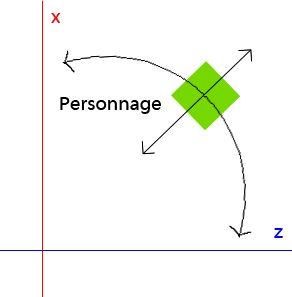
\includegraphics[scale=0.5]{deplac1.jpg}
\caption{Déplacements - première soutenance}
\end{center}
\end{figure}

Une fois le problème du produit matriciel compris et résolu, les déplacements ont pu se faire de façon plus précise : 

\begin{figure}[h]
\begin{center}
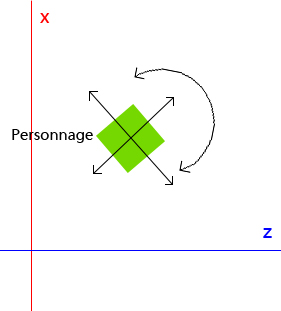
\includegraphics[scale=0.5]{deplac2.jpg}
\caption{Déplacements - deuxième soutenance}
\end{center}
\end{figure}

Après m'être occupé de l'affichage et du déplacement des modèles 3D, il a fallut m'occuper des collisions. Dans le monde du jeu vidéo, les collisions sont une des choses les plus importantes. Si les collisions sont mal gérées, lors d'un combat par exemple, on peut se faire tuer par l'ennemi sans avoir pu le toucher une seule fois. Je suis allé chercher des informations concernant les collisions sur internet. Les résultats ne manquaient pas. De nombreuses techniques sont expliquées. Je n'en ai retenu qu'une seule : celle utilisant des \bsc{Bounding Box}. Cette méthode définit une boîte virtuelle englobant chaque modèle 3D présent dans l'environnement. Ensuite une méthode de détection d'intersection permet de détecter si deux bouding boxe sont entrées en collisions. On peut voir un exemple de bounding box sur l'image suivant, elles apparaissent en trait blanc : 

\begin{figure}[h]
\begin{center}
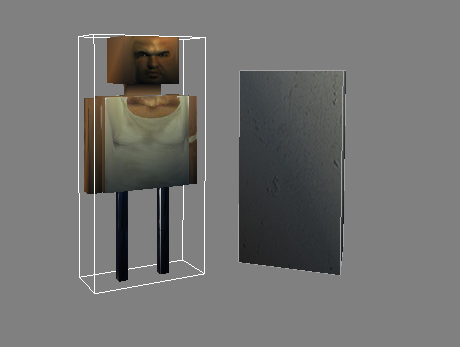
\includegraphics[scale=0.5]{BoundingBox.jpg}
\caption{Exemple de Bounding Box}
\end{center}
\end{figure}

Je n'ai pas eu le temps d'implémenter cette méthode pour la seconde soutenance. Des problèmes apparaissaient au fil du développement.



\subsection{Réalisations}

Pour cette troisième soutenance, nous n'avons pas eu assez de temps pour ajouter de nouvelles fonctionnalités à notre jeu. Nous avons dû en effet répartir notre énergie à nos partiels, nos cours et au projet. En conséquence, peu d'évolution majeures ont fait leurs apparitions entre la deuxième et la troisième soutenance. Dans la suite de cette partie, je détaille le travail que j'ai effectué, seul ou à plusieurs.

\subsubsection{Animations 3D}



Notre deuxième soutenance a vu l'apparition d'un générateur de carte et de l'affichage de carte. La gestion des différents éléments en 3D a aussi été rendue plus simple. Mais il manquait une chose essentielle : l'animation 3D. Les personnages 3D, lors de leurs déplacements, ne sont pas animés. Les jambes, les bras ne bougent pas. Les personnages sont simplement translatés dans l'espace. Ma première tâche a été de réaliser les animations des personnages. Une tâche ardue qui a requis de nombreuses heures de travail. Pour cela, j'ai utilisé le logiciel de modélisation 3D Blender. Il s'agit d'un logiciel libre assez simple qui permet une bonne introduction au graphisme 3D. L'animation des personnages se résume seulement à un pas complet. C'est à dire coordonner le mouvement de chaque membre du corps : l'avancement de chaque jambe et le contre-balancement des bras. Il suffit ensuite de jouer cette animation en boucle pour donner l'impression d'une marche. Chaque type de personnage à son type de marche. J'ai donc animer différement le personnage principale, les gardiens et les autres prisonniers. 

Pour l'affichage et le déplacement des modèles 3D, je me suis heurté à un premier problème. Il faut manipuler des matrices et le produit matricelle pour juste afficher un modèle. Malheureusement, je n'avais pas encore saisie la subtilité du produit matricielle : il n'est pas commutatif. J'ai perdu énormément de temps sur ce point au début. En ce qui concerne l'animation à proprement parler, j'ai rencontré une nouvelle difficulté. Pour la comprendre, il faut comprendre comment un modèle 3D est enregistré. Un modèle est en réalité un squelette sur lequel on vient poser une image, une texture comme on le ferait avec du papier peint. Et c'est ce squelette qui est enregistré en mémoire. Chaque mouvement ou rotation de chaque os de ce squelette est aussi enregistrée pour constituer plus tard une animation 3D. Pour animer le modèle, il faut dire au programme de charger l'état suivant du squelette. Mon problème a été justement de charger la position suivante. Je ne savais pas quelle propriété du modèle utiliser, ou comment faire pour modifier l'état du squelette. \\
Très peu de documentation existe sur Internet. Je n'ai réussi à trouver qu'un exemple issue du site officiel de microsoft. Mais cet exemple n'avait aucune explication ou commentaire. Déchiffrer les lignes de code a été assez ardu. Au fait de mon manque d'expérience en programmation 3D, beaucoup de temps a été nécessaire pour reproduire l'exemple. Une erreur revenait souvent : la même image était chargée sans arrêt. Après de nombreux tests infructueux, j'ai finalement réussi à obtenir une animation complète des personnages.

\newpage

\subsubsection{Création d'une intelligence artificelle}

A ce stade du développement, notre personnage est capable de se déplacer dans son environnement 3D et d'entrer en collision avec les murs, grâce au travail d'Anatole. Faire se déplacer les ennemis a donc été l'étape suivante dans le développement du jeu. La difficulté est de déterminer un chemin aléatoire dans la carte. Il faut que ce chemin soit libre de murs et d'ennemis, pour que le déplacement s'effectue sans encombre. Une fois ce chemin déterminé, il faut trouver un moyen de le faire parcourir par l'ennemi. Pour choisir un chemin aléatoire, nous définissons en premier lieu une distance maximale. Puis nous placons un marqueur à la position de départ de l'ennemi. Ensuite, une direction est choisie au hasard. Le programme suit ensuite cette direction jusqu'à l'intersection suivante, où il choisie une nouvelle direction au hasard. Ce processus est répété tant que la distance maximale n'est pas atteinte. Cela permet d'obtenir un parcours pseudo-aléatoire. 

Vient ensuite le problème du déplacement des ennemis. Nous savons où ils doivent aller, mais nous ne savons pas comment. Etant donné que le déplacement des ennemis ne concernait pas vraiment la boucle de jeu principale, une seule idée nous est apparue, à Anatole et moi. Il s'agissait d'utiliser des processus en parallèle, ou des \bsc{Thread}. Un thread est un outil du \bsc{C\#} qui permet d'exécuter deux actions en parallèles, ou en tout cas en donne l'illusion. Un ordinateur, naturellement, ne peut effectuer qu'une seule chose à la fois. Ainsi les ennemis sont capables de se déplacer de façon aléatoire et autonome, sans ralentir l'exécution principale. 

Mais se déplacer selon un chemin prédéfini en permanence n'est pas très "intelligent" pour une intelligence artificielle. C'est pourquoi Anatole et moi avons implémenté une capacité repérage aux ennemis.  Lorsque notre personnage se situe à une faible distance d'un ennemi et que celui-ci regarde dans la direction du personnage, alors on considère que le personnage est repéré. Dès lors, l'ennemi va poursuivre le héros, jusqu'à la mort de l'un des deux ou si le héros arrive à échapper à la surveillance de l'ennemi. 




\subsubsection{Utilisation d'armes}

Notre jeu dispose maintenant d'ennemis capables de se déplacer et d'un personnage. Il nous manquait encore la possibilité d'utiliser des armes, telles qu'un pistolet ou un couteau. Etant donné que ce point est encore relatif à la 3D, je m'en suis occupé. La première étape a été de modéliser des armes en 3D, avec Blender. Khalis s'en est occupé. Pour qu'un personnage se saississe d'une arme et qu'elle vienne se placer dans sa main, il faut placer un marqueur. Ce marqueur se situe à l'emplacement de la main droite. J'ai donc dû modifier les modèles 3D pour qu'ils intègrent un tel marqueur. Je peux ainsi récupérer la position et l'orientation de la main et y placer l'arme.

Quant à l'utilisation des armes, il a fallu créer deux classes différentes. Une pour les armes dites de corps à corps et une pour celles à distance. Lorsque l'on utilise une arme de corps à corps, la classe correspondante va vérifier si un ennemi se trouve à proximité de l'arme et qu'il se trouve en face du personnage. Si ces conditions sont réunies, alors on considère que l'utilisation de l'arme est positive, c'est à dire qu'elle a touché un ennemi. Déterminer de quel ennemi il s'agit est ensuite simple. Il ne reste plus alors qu'à lui retirer un certain nombre de points de vie. La difficulté de cette méthode se situe dans la détection d'un ennemi. 




\newpage

\subsection{Conclusion personnelle}

A mon entrée en première année à EPITA, j'étais excité de devoir réaliser un projet durant le second semestre. Et au terme de ce projet, je suis toujours autant excité d'avoir eu à le faire. 

Evidemment, ces six mois a vu de nombreux différends entre les quatre membres du groupe. Mais à tout moment nous gardions une bonne cohésion. Une désolidarisation du groupe aurait signifié l'échec du projet. De mon point de vue, ce projet avait pour but premier de nous apprendre à travailler en équipe et non de nous apprendre à mener à terme un projet. 

J'ai été nommé chef de projet en début d'année. Ce rôle incombe de nombreuses responsabilités. J'ai dû axer notre groupe sur un chemin de développement que chaque membre acceptait. Assez passionnant au début, cela devient vite frustrant quand on doit effectuer des choix. 

Pour résumer cette expérience, je dirais que ça a été un plus pour mon futur à EPITA. En tant que chef de projet et membre d'un groupe, ce semestre a été enrichissant. Au lieu de ne rencontrer que des portes ouvertes, nombreuses sont celles à être restées fermées. A chaque nouveau problème, il me fallait trouver un compromis, une solution qui satisfasse toute l'équipe. Et à chaque fois, mes prises de décisions étaient plus rapide. Ayant le plus d'expérience, j'ai souvent plaidoyer en faveur de certaines idées, jugeant celles-ci réalisables ou non. A l'inverse, si nous n'avions rencontrés aucune difficultés, ce projet ne nous aurait pas été profitable. Durant nos années d'études, il y aura de plus en plus de contraintes. Apprendre à les gérer assez tôt est important. Parmi ces contraites, j'entends aussi bien les divergences d'avis que les contraintes techniques imposées par un client. 

\newpage

\section {Anatole Moreau}

\subsection{Récapitulatif des deux premières soutenances}
\subsubsection {Première soutenance}
\underline {Sons}
\par
Si quelque chose m'importe beaucoup dans un jeu, c'est bien la gestion des sons. La qualité sonore m'importe et je suis très pointilleux à ce sujet grâce à ma passion pour la musique. J'ai donc reçu la tâche qui correspond à la gestion des sons. J'ai alors lu un tutoriel sur XNA jusqu’à arriver à la partie son, et me rendre compte... que tout est simplifié avec XNA ! Plus facile encore que FMOD et pourtant bien flexible grâce aux options, la découverte des classes SoundEffect, Song et de la classe statique MediaPlayer était un plaisir pour moi ! Pour commencer, j'ai pris des sons d'une qualité faible mais libres de droits sur internet et je les ai rognés avec Audacity pour éviter l'attente. J'ai placé deux musiques qui jouent le rôle de thèmes dans la boucle principale du jeu pour lancer l'ambiance lugubre d'une évasion de prison.


\underline {Menu, Fenêtre et Jeu}

\par
J'ai eu la chance de travailler sur quelque chose de très concret, visible directement lors de la compilation. C'était un travail de structuration qui fonctionne maintenant correctement, grâce à la classe Fenêtre. En effet, celle-ci contient, comme chaque classe, une méthode Update et une méthode Display. Sauf qu'ici, on switch la valeur d'un attribut de la classe qui contient le contenu qu'il faut charger ou afficher (de type content, une énumération). La fenêtre est donc capable de recevoir un contenu, de le charger, le mettre à jour et l'afficher en faisant à leur tour appel aux fonctions Update et Display de l'objet à utiliser.

\par
Le menu a été le premier rendu visuel du projet. En lui-même, rien de bien compliqué dans un menu: des boutons, une fonction Update qui teste les actions de la souris, et l'appel d'une fonction Fenetre.LoadContent lors d'un clique. J'ai en revanche eu du mal à gérer le mode plein écran comme je le devais. En effet la résolution de l'image était fortement diminuée lorsque l'on passait du mode fenêtré au mode plein écran, et j'ai associé ce problème avec le fait que l'image était de base d'une résolution faible et qu'elle n'était pas faite pour couvrir tout le format d'un écran. Or, il s'avérait que j'ai eu tort, puisque Louis s'est penché sur le problème et a trouvé la faille ! 
\begin{figure}
\begin{center}
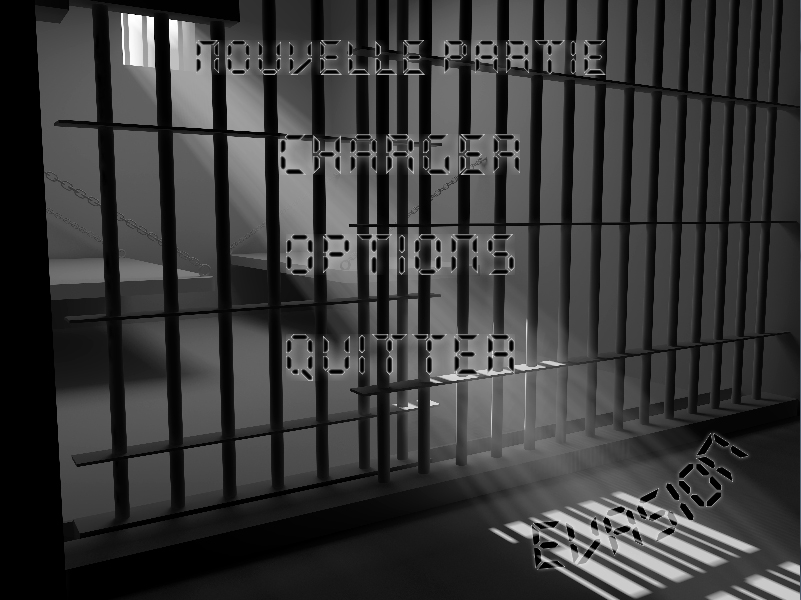
\includegraphics[scale=0.5]{menu.jpg}
\caption{Menu}
\end{center}
\end{figure} 

\par
Pour ce qui est du jeu, j'ai créé les objets nécessaires dans le constructeur (les personnages, le Niveau qui contient les informations de la map en fonction de l'avancée du joueur dans le jeu, les Sons). La boucle principale est faite de manière lisible, le jeu tourne correctement.

\underline{Le site web}
\par
Je me suis désigné pour m'occuper du site web, car c'est un domaine que je connais bien, et dans lequel j'aimerais encore progresser. J'ai alors lu un tutoriel de quelques centaines de pages sur OpenClassrooms d'apprentissage du langage Javascript, pour compléter mes connaissances déjà acquises de HTML, CSS, PHP et SQL pour modeler un site bien personnel, sans aucun appel à des modules externes ou logiciels. Le thème du site est à l'image du jeu, sombre, et évoque la prison à plusieurs reprises (bouton de menu, image d'en-tête). J'ai pu utiliser les connaissances apprises au cours de ce tutoriel dans le site à travers la création d'une galerie d'images, et d'un cadre "A propos", qui s'affiche sur presque toutes les pages du site. J'ai implémenté un système d'ajout de posts, avec un upload automatique de fichiers en PHP sur le serveur.
\newpage
\begin{figure}
\begin{center}
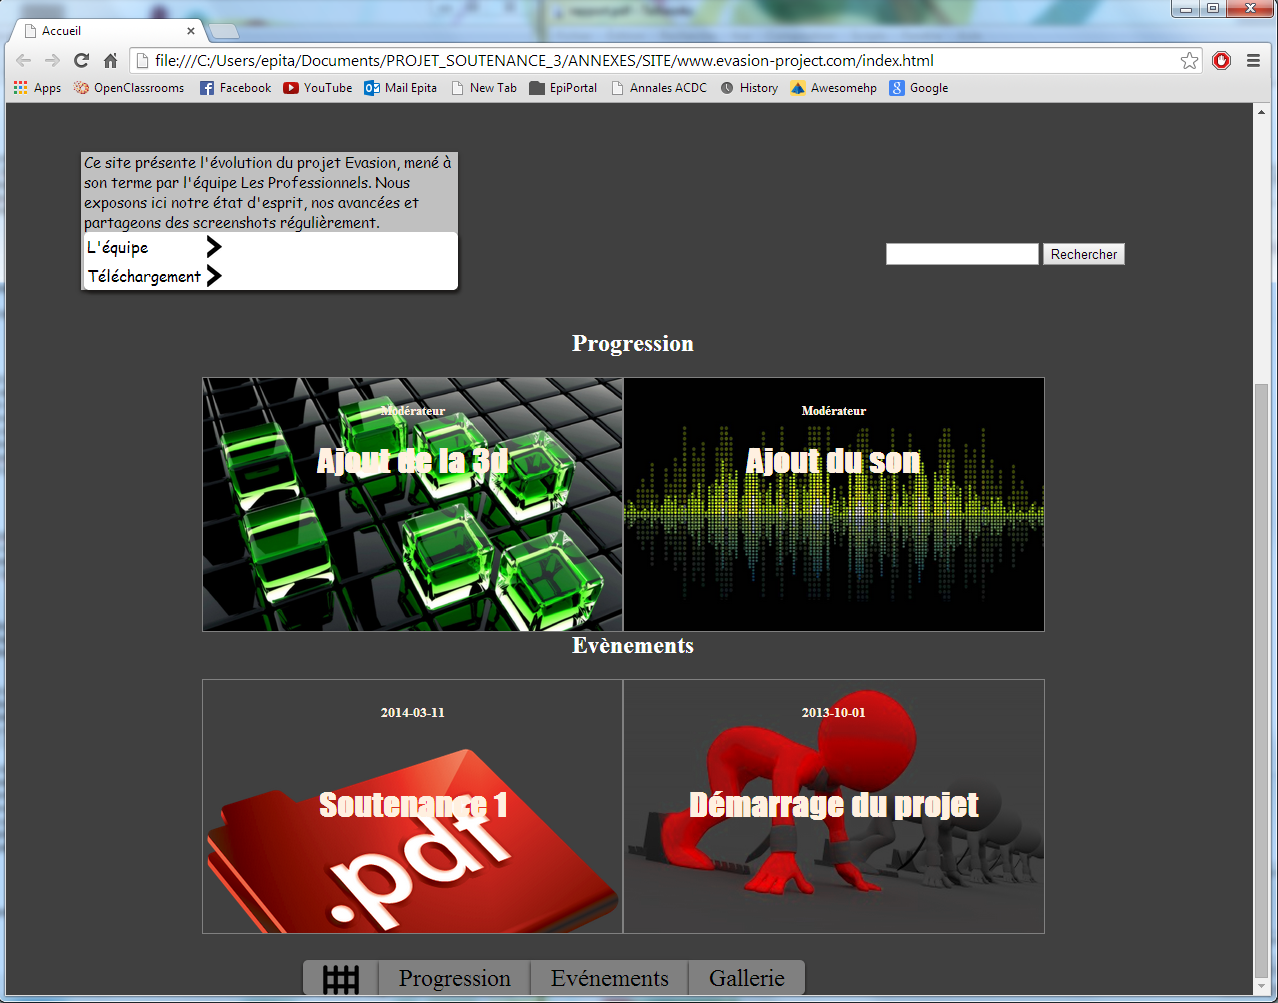
\includegraphics[scale=0.4]{Site.png} 
\caption{Site}
\end{center}
\end{figure}

\subsubsection {Deuxième soutenance}
\underline{Jeu.cs}
\par
Une grande partie de mon travail était déjà entamée grâce a la même structure qui se répète dans chaque classe de notre projet, c’est-à-dire l’existence d’une fonction Load, une fonction Update, et une fonction Draw. J’ai donc implémenté ces trois fonctions en utilisant des listes d’éléments déclarées comme attributs de la classe. Le jeu appelle à leurs tours les trois fonctions de chaque éléments de ces listes, et tout s’emboite correctement. Le rendu visuel a été visible grâce au travail graphique de Louis, Lenny et Khalis sur Blender et Photoshop. Toute la structure du code est ainsi visible dans ce fichier, qui est la base du déroulement du jeu. On y retrouve la boucle principale, qui gère les différents évènements du clavier. Tout ce qui concerne la caméra a été fait par Louis. Les boutons actuellement gérés permettent de : \\
- Mettre le jeu en pause ; \\
- Quitter le jeu de force ; \\
- Déplacer le(s) joueur(s) ; \\
- Changer l’angle de vision du/des joueur(s) ; \\
- Monter/Descendre la caméra, qui ne se déplace pas automatiquement avec le décors ; \\
- Arrêter /Reprendre la musique d’ambiance ; \\
Le jeu a également hérité d’une fonction chargerNiveau qui traite chaque information d’un fichier texte pour créer chaque élément de la carte un par un en les rajoutant aux listes initialisées au préalable.
\newpage
\underline {Editeur de map} 
\begin{figure}
\begin{center}
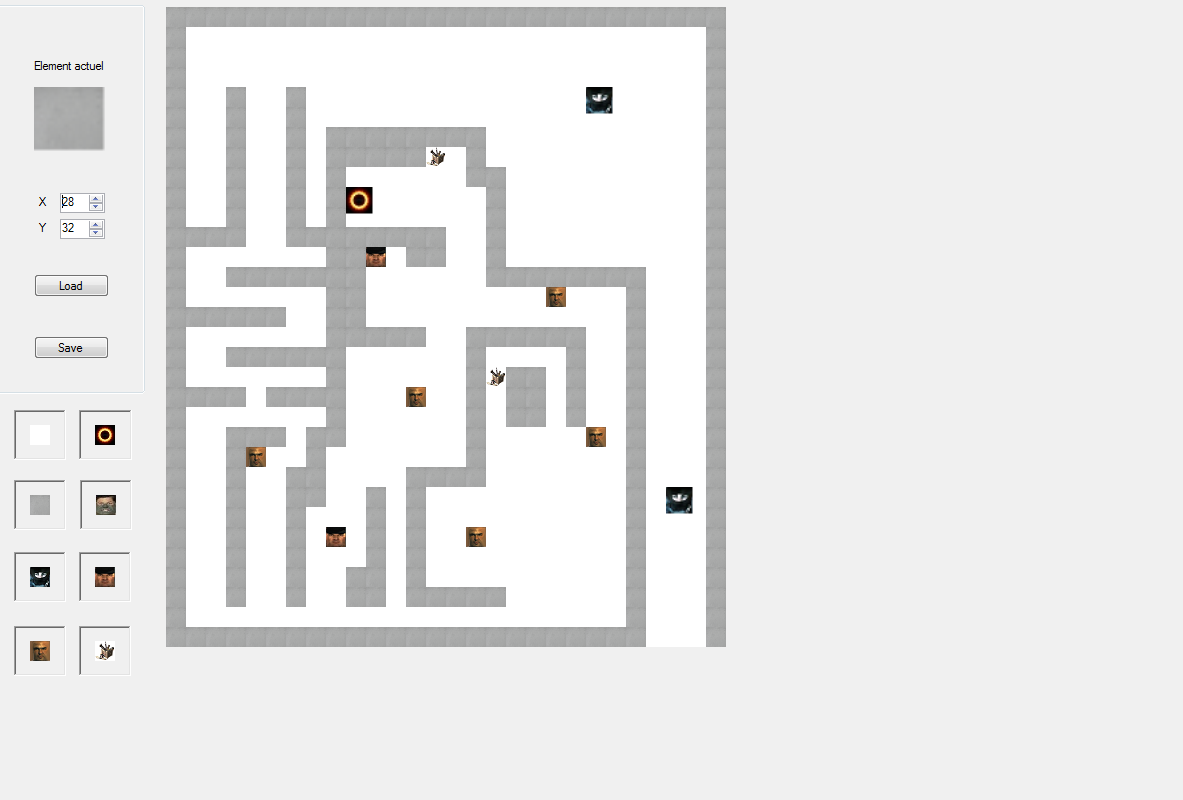
\includegraphics[scale=0.5]{editeur.png}
\caption{Editeur de map}
\end{center}
\end{figure}
\par
Lorsque le rendu d’affichage d’un sol et de murs était correct, il a fallu implémenter un rapide moyen de créer des niveaux pour la diversité du jeu. J’ai donc pris l’initiative de faire un petit éditeur de map, que l’on a rendu accessible aux utilisateurs pour rendre le jeu plus flexible en attendant sa finition. Il offre un terrain aggrandissable et réductible, et des éléments a y insérer. On y voit par exemple des points de spawn qui décident aleatoirement de la position d’apparition du joueur, des ennemis qui seront les éléments cles de la difficulté du niveau, des murs, caisses de munitions. Le tout doit être stocké dans un fichier texte placé dans le répertoire des ressources du jeu. Cet éditeur nous a permis de concevoir deux cartes qui s’apparentent a l’intérieur d’une prison, mais tous les éléments ne s’affichent pas encore dans le rendu bien qu’ils soient traités par une fonction qui charge les éléments de la carte dans le jeu, car l’avancement graphique n’est pas terminé à cet instant. Ainsi, les munitions placées sur une carte n’afficheront rien. La sauvegarde s’effectue simplement à l’aide d’une énumeration d’éléments, chacuns représentés par un int non signé, que l’on écrit sur le fichier texte, avant de le lire dans l’autre sens depuis Jeu.cs qui charge le niveau.


\underline {Mode multijoueur} 
\par
Khalis et moi avons fait la connaissance des viewports a l’occasion de l’implémentation d’un mode multijoueur. Bien que les objectifs ne soient pas encore disponible, le partage d’écran est fini, avec l’acquisition de connaissances concernant les viewports. On a rencontre des difficultés au niveau du plein écran et de la barre de séparation, avant de constater que cela venait d’une mauvaise compréhension des viewports. Ce fut donc l’essentiel de notre tache. On a rencontré pas mal de problèmes pour le passage en plein écran, notamment pour l’affichage du HUD (Head-Up Display) (les vies, la barre de séparation) et on a remanié la surcharge de la fonction draw pour parvenir à nos fins. 
\begin{figure}
\begin{center}
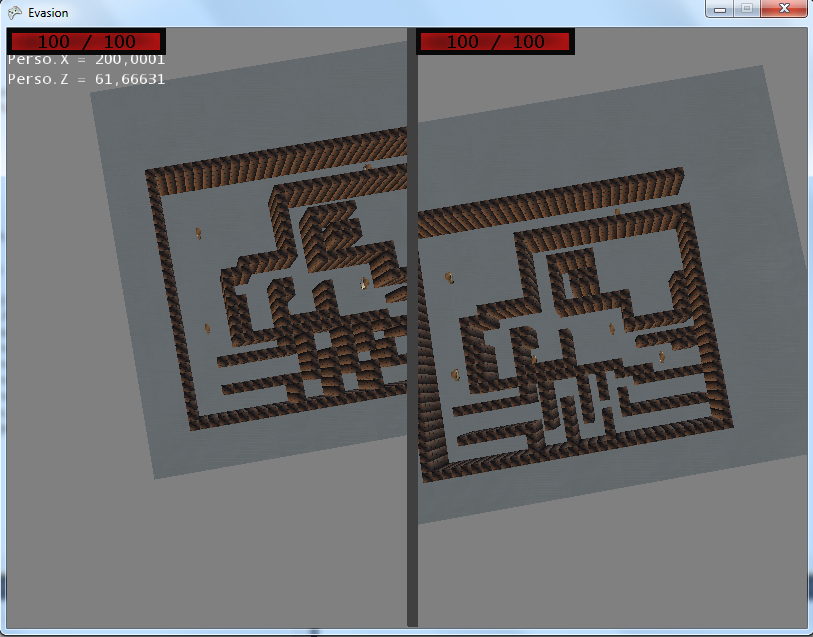
\includegraphics[scale=0.7]{multi.png}
\caption{Mode multijoueur}
\end{center}
\end{figure}
\underline {Site web} 
\par
Le site web a subi une amélioration nette de la clarté du code, accompagne d’un changement esthétique. Avec Khalis à l’appui, le travail a été plus structuré et on a pu gagner en flexibilité. On a déplacé la barre de menu en haut de la page et on a dessiné un pied de page. Les divisions qui étaient placées de manière désordonnée ne le sont plus, et chaque classe de html a sa propre utilisation.

\subsection{Taches accomplies pour la troisième soutenance}
La soutenance finale devra présenter le projet finalisé, c'est-à-dire à l'état de produit fini. Il est alors naturel de reprendre les premières esquisses du projet.
Dans notre cas, le but initial était de produire un jeu agréable pour l'utilisateur, qui comportait des technologies qui nous étaient alors étrangères. La maîtrise de ces technologies a été acquise au cours des soutenances précédentes. Cette fois-ci, nous avons donc utilisé notre temps pour finaliser le jeu, éviter qu'il comporte des erreurs, rendre le déroulement du jeu logique, ainsi que des touches instinctives pour ne pas gêner le joueur. Voici donc la liste exhaustive des tâches que j'ai réalisées pour cette dernière soutenance.
\subsubsection {Site web} 
Le site web a été remis en forme graphiquement grâce à Dreamweaver. Cet outil m'est familier, et son utilisation est très intuitive grâce à un rendu visuel qui répond au critère : What You See Is What You Get (WYSIWYG). Dreamweaver montre visuellement le lien direct entre le code et son rendu. Cela a permis à Khalis de travailler sur ce logiciel avec moi, ce qui a facilité la compréhension du code entre nous deux. En plus de cela, le site a été rendu international avec l'ajout d'un choix de langage qui comporte le français et l'anglais.
\subsubsection {IA} 
Les ennemis était inertes jusqu'ici. Leur donner un aspect vivant a été simplifié par le fait qu'il s'agissait de gardes de prison. L'intelligence artificielle dont ils sont dotés est donc capable de leur faire exécuter deux actions : marcher, repérer une anomalie et combattre. A chaque instant, une fonction teste leur champ de vision et change un booléen (valeur pouvant être à l'état vrai, ou l'état faux) représentant leur mode d'action : ils peuvent soit être passifs et continuer leur marche, soit être actifs et tenter de tuer le fugitif en lui tirant dessus. Le pistolet dont ils sont munis ayant une certaine portée, la trajectoire du tir est un lancé aléatoire et la gestion de la collision entre le tir et un joueur se fait de manière linéaire : le tir est considéré comme ne changeant pas de hauteur. S'il rencontre un mur ou un joueur, le teste linéaire s'arrête. Une petite difficulté a été rencontrée à ce niveau : le repérage d'ennemi se fait en fonction de la rotation du personnage, ce qui induit l'utilisation d'une petite formule mathématique. De plus, les ennemis sont capables de s'orienter seuls dans la prison en choisissant une direction, qui tournera leur rotation de 90, 180 ou 270 degrés. Ils doivent donc savoir repérer un mur à proximité pour savoir quand changer de direction. La direction est aléatoire entre les directions possibles. Le programme chargé de déplacer les ennemis est en fait indépendant de la boucle principale du jeu. Il s'exécute parallèlement à cette boucle. Ce type de programme est appelé Thread.
\subsubsection {Réseau}
Khalis et moi avons aidé Lenny qui avait entamé la recherche sur le réseau. Un tp réalisé au cours de l'année nous a donné les outils abstraits pour comprendre le fonctionnement du réseau impliquant l'utilisation d'un serveur et de clients. Le serveur est un programme qui tourne séparément du programme des clients (le jeu). Ce serveur contient la mise à jour des éléments de la carte. Il contient un Thread qui envoie ces données et reçoit les données de chaque joueur séparément. Le client affiche les données envoyées par le serveur et envoie les données relatives au joueur. Pour réaliser cela concrètement, Khalis et moi avons examiné un tutoriel de MSDN, expliquant étape par étape comment faire fonctionner le système : comment connecter le client au serveur, comment envoyer des données de l'un à l'autre.
\subsubsection {HUD} 
\par
Le confort visuel s'est accentué grâce à plusieurs ajouts dans le Head Up Display (HUD). Le premier ajout a été celui des objectifs, qui s'affiche à la manière d'une liste en écriture blanche. Les objectifs sont chargés dans le fichier texte qui représente le niveau sur lequel le joueur joue. La liste est exhaustive et diminue de hauteur à chaque fois qu'un objectif est atteint. 

\par
Le deuxième ajout a été celui de l'inventaire du joueur, qui démarre avec un couteau uniquement. Celui-ci peut se remplir si le joueur trouve des objets disposés sur la carte du jeu, comme un pistolet.

\subsubsection {Options} 
Les options ont été implémentées pour laisser au joueur un sentiment de maîtrise, et rendre le jeu plus flexible. Ainsi, les options proposent un réglage du volume, l'activation ou non du mode plein écran, et la langue du jeu.

\subsubsection {Logique du jeu} 
Ce que j'appelle la logique du jeu, c'est la manière d'indiquer au joueur les évènements qui arrivent. Je me suis occupé de dessiner plusieurs écrans pour indiquer la défaite ou la victoire du joueur. En mode multijoueur par exemple, lorsqu'un joueur meurt, l'autre joueur peut continuer de jouer.

\subsubsection {Sauvegarde et chargement} 
Encore une fois, je me suis servi de la sérialisation pour sauvegarder des informations concernant la partie en les condensant en chiffres et en lettres : le niveau actuel du joueur ainsi que le nom de la sauvegarde sont stockés dans un fichier texte qui se situe dans un dossier particulier. Le chargement s'effectue en ouvrant le fichier sélectionné par l'utilisateur. 

\subsubsection {Collisions} 
Le système de collisions n'était pas au point lors de la deuxième soutenance. Comme je m'occupais de la classe Niveau, qui gère l'affichage et la création du décors, j'ai utilisé un système basique de collisions fait à la main dans cette même classe. Le rendu n'est pas parfait car il ne gère pas la rotation du personnage qui se déplace, mais il est convenable et n'enlève pas de satisfaction de jeu.

\subsection{Conclusion personnelle}
Un projet mené avec un groupe est une expérience très riche. C'est à la fois un moyen de partager ses expériences et ses compétences, et un moyen d'apprendre à s'adapter aux autres. C'est aussi une expérience personnelle, car certaines minces tâches ne peuvent  se faire que par une seule personne sous peine de mésentente. C'est pourquoi chaque membre du groupe est responsable de l'entier aboutissement du projet, et c'est ce qui mène à des conflits au sein du groupe. 

\par
C'est là qu'intervient l'importance de la hiérarchie : le chef du groupe peut revenir sur des décisions et résoudre les problèmes liés au manque d'expérience de chacun. Si une partie du projet tarde à s'achever, il peut demander à un membre plus expérimenté de prendre le relais sans avoir besoin d'être approuvé. Même s'il ne prend pas la bonne décision, son avis est important et résout le problème du nombre pair du groupe, qui pourrait impliquer des avis partagés trop équitablement sur des problèmes. 

\par
Un groupe de projet de ce genre permet aux membres de réaliser un débat d'idées pour introduire le projet. C'est ainsi que chacun dévoile sa personnalité, et connaitre la personnalité des personnes avec lesquelles on travaille est un atout qui permet une meilleure compréhension entre les membres, un gain de temps, et une motivation plus  importante. Si notre projet personnel a démarré sur des disparités au niveau de l'expérience de chacun des membres, il en revient une égalité du potentiel de chacun, un objectif partagé, un apprentissage collectif.

\par
Le projet était libre au niveau de la réalisation, c'est pourquoi nous avons appris à fixer nos propres contraintes. Mais le temps nous était fixé d'emblée. Nous avons expérimenté le problème d'organisation, qui engendre un retard temporel. Il en ressort pour ma part qu'un groupe a besoin d'un meneur capable de décider : "Rendez vous ici de telle heure jusqu'à telle heure". Si ce rendez-vous est fixé à l'avance, lorsque le moment arrive, nous sommes déjà préparés mentalement. Dans le cas contraire, le travail est moins productif, la lassitude nous gagne vite. Cela s'explique par le fait que nous ne nous sentons pas obligés de travailler. 

\par
Une dernière conclusion personnelle est la limite d'avidité à se fixer. J'ai appris qu'il me fallait des limites très fermes pour éviter que je m'arrête sur du travail supplémentaire facultatif. La liberté de création est inspirante, mais aussi dangereuse. Les objectifs doivent être revus à la baisse si ceux-ci se présentent comme difficiles à atteindre.



\newpage

\section{Khalis Chalabi}
\subsection{Récapitulatif des deux premières soutenances}
\subsubsection{Soutenance 1}
Pour cette première soutenance je devais implémenter plusieurs classes, faire bouger un personnage 3D et je m'étais fixé comme objectif acquérir des bases en développement web pour pouvoir commencer à développer le site de notre jeu vidéo avec l'aide d'Anatole. Au début de l'année mon niveau en programmation n'était pas suffisant pour pouvoir réaliser les tâches que mon groupe m'avait confiées. Mon travail dans ce projet a donc débuté avec un très grand travail de recherche. Les tutoriels et les aides trouvés sur Internet, mais surtout, les membres de mon groupe m'ont permis d'élargir mes connaissances en informatique.


Les TPs réalisés au cours de l'année m'ont permis d'implémenter les classes Personnages, Objets et Décors sans faire plus de recherches. Cependant, faire déplacer un personnage 3D à l'aide du clavier me dépassais complètement. Je me suis donc mis à la recherche d'un tutoriel qui allait pouvoir me permettre de réaliser cet objectif. Le site du Zéro étant un site complet et détaillé pour les débutants, je me suis rendu sur ce site pour commencer. J'ai pu y trouver un tutoriel expliquant le développement de jeu vidéo avec XNA. A première vue ce tutoriel semblait parfait pour moi vu que notre jeu vidéo devait fonctionner sous XNA. Les explications étaient plutôt simples si l'on avait déjà quelques bases en C\# ce qui était mon cas. Le tutoriel débutait avec un rappel de ce qu'était XNA et ce qu'on pouvait faire avec ce Framework. Puis il expliquait l'utilisation des sprites, et pour finir, comment faire interagir une image avec le joueur. Cependant, il est ici question de 2D or notre jeux vidéo est un jeu en 3D. Malgré cela, ce tutoriel m'a grandement aidé pour comprendre comment faire bouger une image avec les touches du clavier ou une souris. J'avais donc enrichi mes connaissances en programmation et pouvais, dorénavant, commencer à essayer de faire bouger mon personnage 3D.

Lors de la 2ème soutenance il est obligatoire de présenter un site web. Un membre de notre groupe, Anatole, possédais déjà les connaissances nécessaires pour la création d'un site web. Cette partie m'intéressais je lui ai donc proposé de nous occuper du site web ensemble. Cependant, encore une fois, mes connaissances étaient légères. Le site du Zéro me fût encore d'une très grande aide car c'est grâce à celui-ci que je pu apprendre les bases de HTML5 et de CSS3 deux langages webs utilisés majoritairement pour la création de site web.

Mes recherches finies, j'essayais de mettre en pratique ce que j'avais appris. Comme je vous l'ai précisé dans les paragraphes précédents, mais sans entrer dans les détails, j'étais chargé d'implémenter les classes Personnages, Objets et Décors. Parmi les tâches qui m'étaient attribuées j'ai décidé de commencer par celle-ci car grâce aux TPs, je savais ce qu'était une classe et comment cela fonctionnait. Cependant il n'y avait pas juste trois classes à implémenter mais beaucoup plus! En effet la classe Personnage était la classe mère et elle possédait des classes filles : la classe Ennemi, la classe Joueur ainsi que la classe PNJ (personnages non jouables). Et il en était de même pour les classe Objets et Décors elles possédaient chacune plusieurs classes filles. La classe mère, Personnages, et ses classes filles furent les plus longues et les plus dures à coder. Elles comportaient plusieurs fonctions et les constructeurs étaient assez longs. Après avoir bien compris la logique les classes Objets et Décors ainsi que leurs classes filles ne furent pas très difficile à implémenter.

Le déplacement du personnage 3D fût la tâche la plus difficile à exécuter vu qu'il fallait interagir avec le joueur et que ce n'était pas une notion que nous avions abordé en TP. Comme je vous l'ai dit précédemment j'ai suivi un tutoriel sur le site du Zéro. Le tutoriel était destiné à un jeu en 2D mais cela ne changeait pas grand-chose au déplacement du personnage en 3D. Il faut juste comprendre qu'en 3D nous utilisons un modèle et qu'en 2D ce sont des sprites. Pour que l'utilisateur puisse contrôler les déplacements du personnage à l'aide du clavier, il suffisait de récupérer l'état du clavier et, en fonction des touches qui sont enfoncés, faire varier la position du personnage 3D ainsi que sa vitesse. Après m'avoir occupé de cette partie il était donc possible de diriger le personnage principal à l'aide des touches directionnelles.

Voici donc, le travail que j'ai fourni pour cette première soutenance. Un travail qui ne fût pas des moindres mais qui m'apporta beaucoup en ce début d'année.

\subsubsection{Soutenance 2}
\par
Nous sommes maintenant à un peu plus du milieu de l'année et mes connaissances ainsi que mon niveau en informatique sont un peu plus développés. Cependant, pour cette deuxième soutenance, il m'a encore fallu mener un travail de recherche. Parmi les tâches qui m'incombait, les graphismes et le mode multijoueur étaient des tâches complexes étant donné que je ne savais pas par où commencer.  

\par
Le graphisme fût une des tâches les plus difficiles à réaliser car il fallait que j'utilise deux logiciels avec lesquels je n'avais jamais travaillé : Photoshop et Blender. Nous faisons un jeu en 3D donc il ne suffisait pas d'importer des sprites et des textures avec XNA comme pour un jeu en 2D. Louis a créé ce qu'on appelle des modèles avec l'aide du logiciel Blender. Ce logiciel permet, entre autre, de modéliser des images en 3D. Nous avions donc la forme principale de nos personnages, il fallait ensuite les personnaliser (lui faire porter des vêtements, lui faire un visage...) Il nous a d'abord fallu découper notre modèle pour obtenir un patron car pour personnaliser le personnage il faut appliquer une texture sur chacune des faces du modèle.
\newline

\newpage

\begin{figure}[t]
\begin{center}
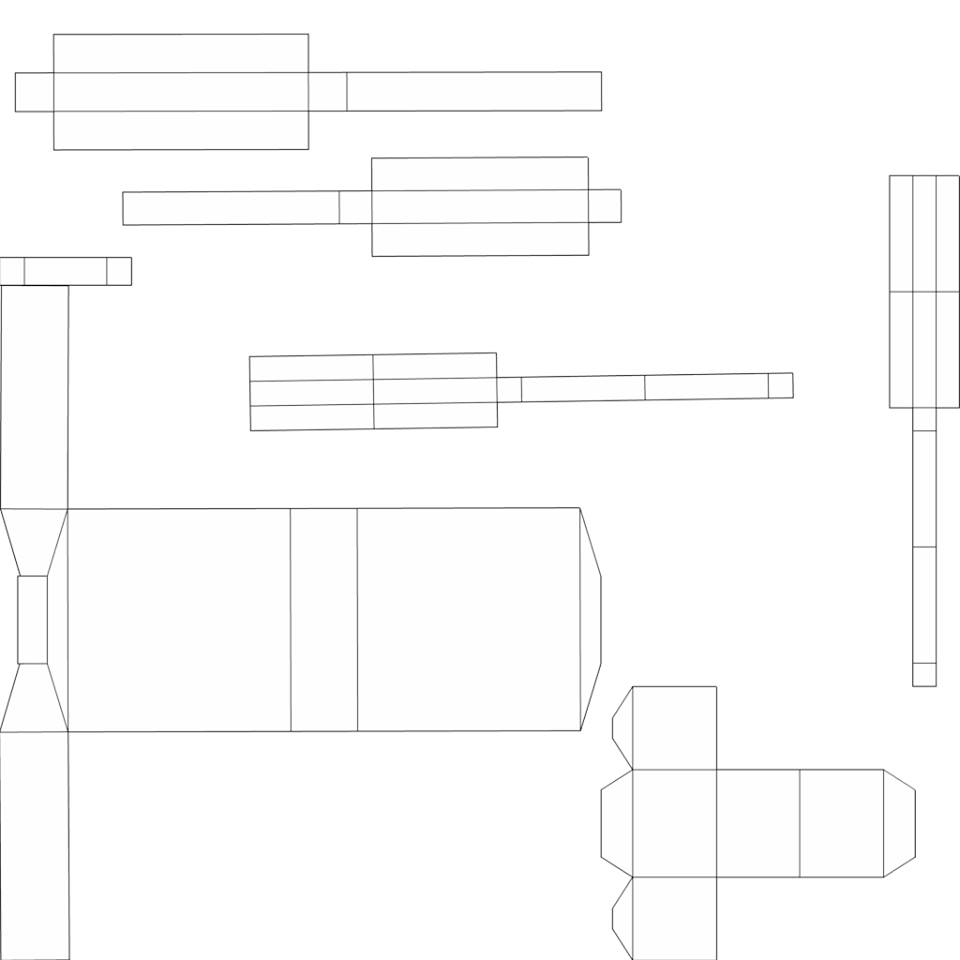
\includegraphics[scale=0.3]{decoupe.jpg}
\caption{Patron du personnage}
\end{center}
\end{figure}


\par
Pour découper notre modèle nous avons utilisé Blender, il fallait découper les faces mais en faisant attention d'en garder une qui soit rattacher aux autres. Imaginez la découpe d'un cube nous a beaucoup aidé. Une fois le modèle complètement découpé nous obtenons l'image ci-dessus. Vous avez peut-être l'impression que cela ne ressemble à pas grand-chose mais en reconstruisant le patron vous obtenez bien le modèle de notre personnage. En haut à gauche de l'image vous avez ses deux bras, juste en dessous et sur la droite ses deux jambes, la plus grosse figure correspond au haut du corps (torse, dos, cou...) et enfin tout en bas à droite sa tête. Une fois ce travail fait il fallait donner l'aspect que nous voulions au personnage. Pour cela j'ai dû utiliser le logiciel Photoshop car pour chaque face du patron il faut comme je vous l'ai dit précédemment une texture. Je me suis occupé de faire le personnage principal ainsi que les gardiens de prison. Je sélectionnais une image qui me plaisait sur Internet puis je prenais la partie qui m'intéressait grâce aux fonctionnalités de Photoshop. Par exemple pour faire le dos du gardien j'ai choisi une image de gardien de prison vu de dos puis j'ai rogné l'image de façon à avoir que le haut de l'uniforme. La difficulté dans cette partie était que je n'avais jamais utilisé Photoshop donc j'ai dû découvrir ce logiciel au fur et à mesure. Lorsque j'avais des problèmes je me renseignais sur Internet ou demandais de l'aide à Louis qui connaît plutôt bien ce logiciel. M'occuper du design des personnages m'a donc demandé beaucoup de temps. Je devais faire de nombreux tests pour obtenir ce que je voulais.
\newline

\begin{figure}[htbp]
\begin{minipage}[c]{.45\linewidth}
\begin{center}
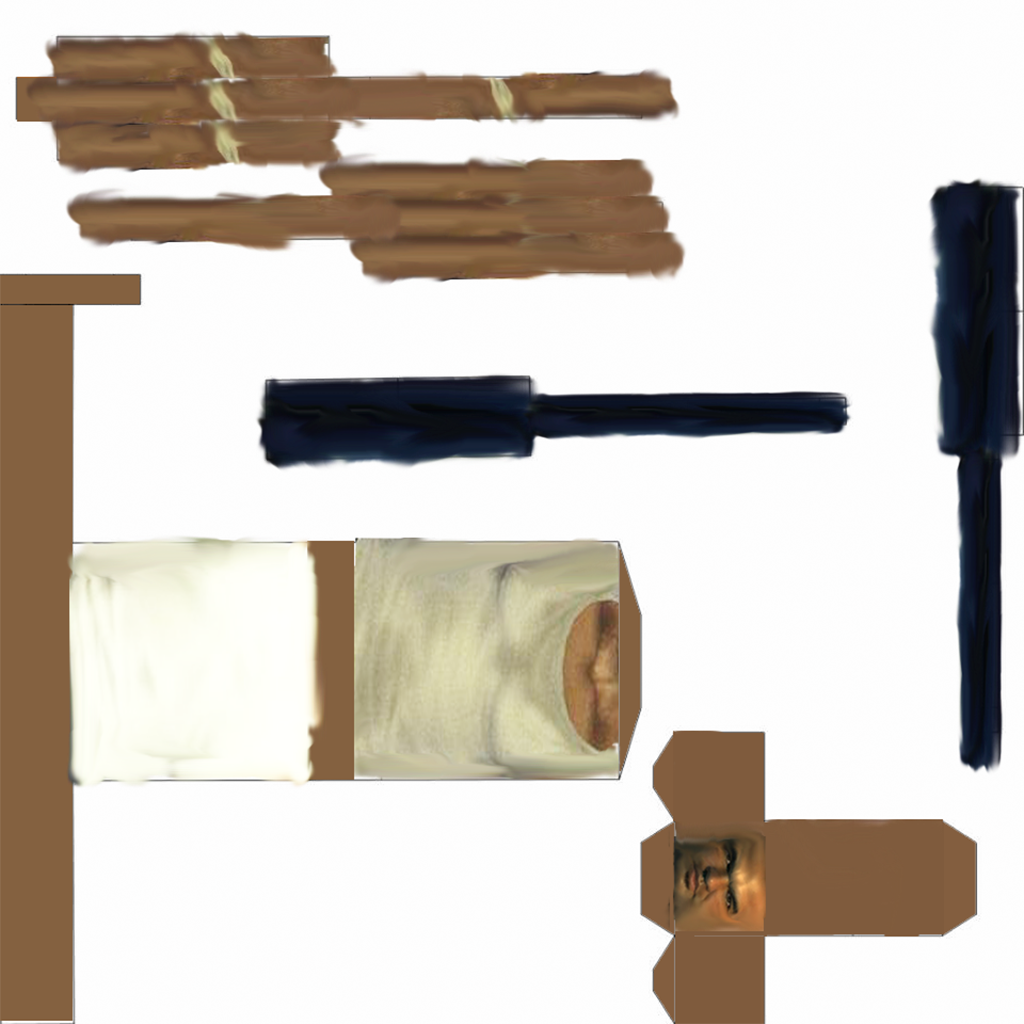
\includegraphics[scale=2]{michaelphotoshop.png}
\caption{Texture personnage principal}
\label{fig:michaelphotoshop}
\end{center}
\end{minipage}
\hfill
\begin{minipage}[c]{.45\linewidth}
\begin{center}
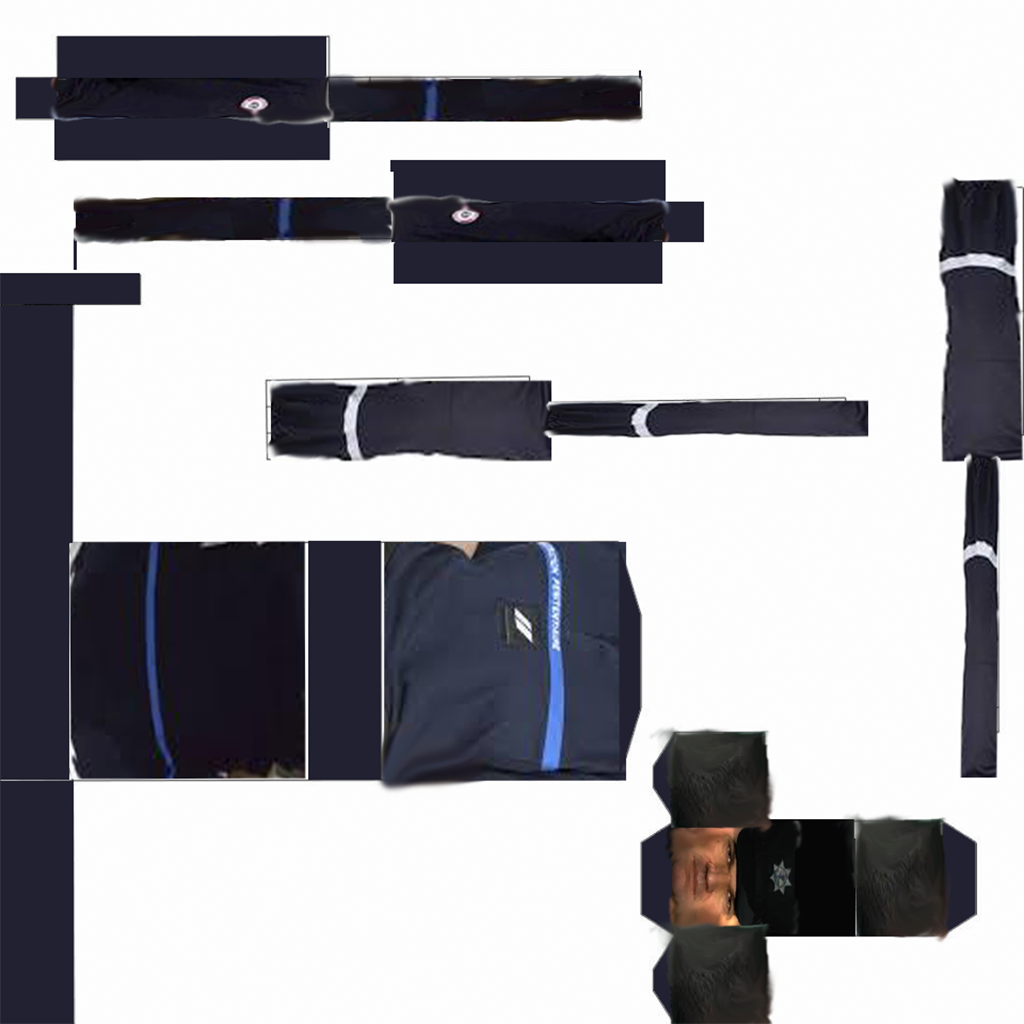
\includegraphics[scale=2]{bellikphotoshop.png}
\caption{Texture gardien de prison}
\label{fig:bellikphotoshop}
\end{center}
\end{minipage}
\end{figure}

\par
Une fois que j'avais fini d'appliquer des textures au patron, j'importais l'image sur Blender pour pouvoir vérifier l'aspect de mon personnage parce qu'avec le patron, comme vous pouvez le voir, on ne s'en rend pas compte. Je regardais l'aspect de mon personnage à chaque modification pour pouvoir éviter de tout recommencer si cela ne me plaisait pas.
\newline

\begin{figure}[htbp]
\begin{minipage}[c]{.45\linewidth}
\begin{center}
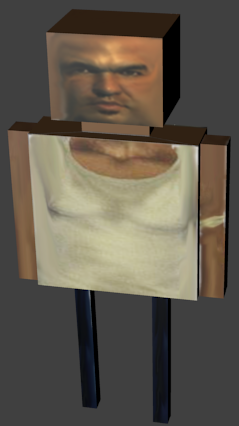
\includegraphics[scale=0.6]{michael.png}
\caption{Personnage principal}
\label{fig:michael}
\end{center}
\end{minipage}
\hfill
\begin{minipage}[c]{.45\linewidth}
\begin{center}
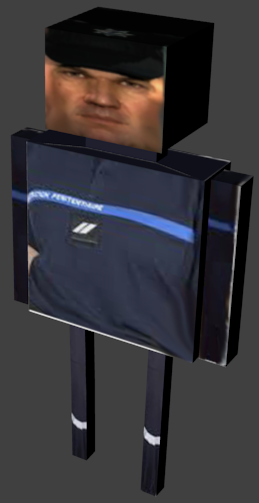
\includegraphics[scale=0.5]{bellik.png}
\caption{Gardien de prison}
\label{fig:bellik}
\end{center}
\end{minipage}
\end{figure}

\par
Une fois le premier personnage fait le deuxième fût plus simple à faire car j'avais pu m'habituer à Photoshop et à Blender. Le plus facile dans cette partie fût la réalisation du mur de la prison. Étant donné qu'en 3D un mur est juste un rectangle le découpage est plutôt simple par rapport au découpage du modèle du personnage. Il suffisait ensuite d'importer l'image d'un mur dans Photoshop puis de légèrement la modifier. Cela nous a donc permis d'avoir les principaux personnages et le début du décors ce qui est une grande avancée car notre jeu vidéo commence enfin à ressembler à un jeu vidéo.

\par
Comme dans la plupart des jeux vidéo, notre personnage possède une barre de vie. Cette dernière se vide en fonction des dégâts reçus et peut se remplir si le personnage se soigne. Elle possède en son centre un nombre qui permet de connaître le nombre de points de vie actuel sur le nombre de points de vie maximum. Pour créer cette barre de vie j'ai implémenté une nouvelle classe nommée ''BarreDeVie''. Avant de commencer à coder, j'ai tout d'abord créé le design de ma barre de
vie à l'aide de Photoshop. J'ai dû créer deux textures : la barre de vie et sa bordure. Une fois cette étape réalisée j'ai pu commencer à implémenter ma classe. Ce ne fut pas très long, la classe ne contenait qu'un constructeur et 4 fonctions. La première fonction me permettait d'ajuster la barre de vie de telle sorte que les points de vie ne soit pas négatifs ou qu'ils ne dépassent pas la valeur maximale définie. Ensuite une fonction qui mettait à jour la barre de vie par rapport au niveau de santé du personnage. Puis pour finir les deux fonctions les plus difficiles. Celle qui permet de réduire la barre de vie normalement et celle qui la dessine dans les bonnes proportions. En effet, lorsque les points de vie diminuaient ou augmentaient la totalité de la barre (le fond rouge ainsi que la bordure) diminuait mais se rapetissait également jusqu'à devenir extrêmement fine et minuscule! De plus elle se dessinait dans de mauvaises proportions car elle prenait toute la longueur de l'écran. Pour régler ces problèmes j'ai utilisé deux surcharges différentes de la fonction ''Draw'' une pour la bordure et l'autre pour le fond. L'affichage du nombre de point de vie est tout simplement possible avec l'utilisation d'un ''SpriteFont''. Pour que tout s'affiche correctement il ne manquait plus qu'à déclarer, initialiser, charger et dessiner la barre de vie dans la classe ''game''.

\begin{figure}[h]
\begin{center}
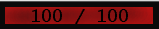
\includegraphics[scale=1.5]{Barredevie.png}
\caption{Barre de vie}
\end{center}
\end{figure}

Un de mes objectifs pour cette deuxième soutenance était de commencer à implémenter un mode multijoueur. Je pense que je m'en suis plutôt bien sorti car il est pratiquement fini (on peut donc dire que je suis légèrement en avance sur cette partie la). Je ne savais pas par où commencer, j'ai dû faire quelques recherches pour comprendre comment débuter. Je voulais faire un mode multijoueur avec un écran scindé où les joueurs verraient chacun leur personnage. J'ai donc suivi un tutoriel sur Youtube qui expliquait comment scindé un écran en deux. Il y a une classe nommée ''Viewport'' qui facilite justement la division de l'écran. Il suffit juste ensuite de copier ce qui se trouve dans l'écran de gauche dans celui de droite. Bien sur le tutoriel était pour un jeu en 2D il m'a donc fallu tester et modifier certaines choses pour que cela fonctionne. Anatole m'a aidé pour cette partie car je ne trouvais pas toute les solutions sur Internet. Pour que la séparation soit nette, j'ai créé une texture avec Photoshop que j'ai ensuite importé avec XNA. Il est donc plus facile de distinguer les deux écrans et cela améliore le design de notre jeu vidéo.
\newpage
\begin{figure}
\begin{center}
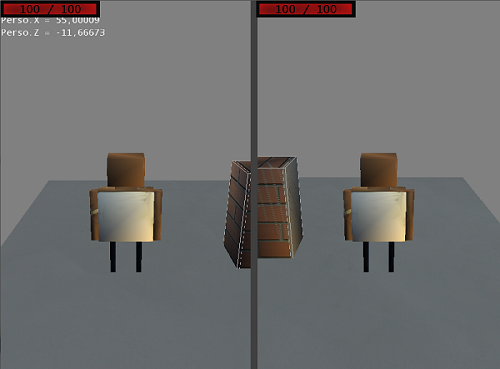
\includegraphics[scale=1]{Multijoueur.png}
\caption{Mode multijoueur}
\end{center}
\end{figure}

Chaque joueur a son propre personnage, sa propre barre de vie ainsi que sa propre camera. L'essentiel du mode multijoueur est donc fait, il ne manquera plus qu'à l'améliorer. Pour finir, j'ai créé un bouton multijoueur dans le menu d'accueil qui permet au joueur de choisir son mode de jeu : le mode solo ou le mode multijoueur.

Nous avions déjà un site web lors de la première soutenance, mais pour la deuxième nous avons décidé de modifier le design du site ainsi que la clarté du code comme Martin nous l'avait demandé. C'était à Anatole et moi-même de nous occuper de cette tâche. J'ai, avant tout, refait le design du site en faisant un croquis sur une feuille de papier. Puis j'ai relu une partie de notre code pour le modifier et l'améliorer.
\\
\\


Le travail fourni pour cette soutenance nous a vraiment fait avancé et progressé. Notre jeu ressemble de plus en plus à un véritable jeu vidéo.

\subsection{Tâches accomplies pour la troisième soutenance}
Pour la soutenance finale j'ai travaillé sur les mêmes tâches que celle de la deuxième soutenance excepté en ce qui concerne le réseau. Mis à part le réseau, notre travail pour cette soutenance est en fait un travail de finalisation et d'amélioration et non plus de création.

J'ai donc continué à m'occuper tout d'abord des graphismes pour avoir un joli rendu à l'écran. Les armes et certains éléments du décor étaient manquants. Cette partie-là ne m’a pas pris beaucoup de temps car je maitrisais assez bien Photoshop et Blender maintenant. Je me suis chargé de faire un plafond en reprenant le model du sol que nous avions mais en changeant la texture. Nous avons décidé de faire deux armes : un couteau assigné par défaut au personnage et un pistolet qu’il devra trouver et ramasser dans la prison pour pouvoir l’utiliser. Pour le pistolet et le couteau j’ai dû créer de nouveaux modèles avec le logiciel Blender et leur appliquer à chacun une texture, à l’aide de Photoshop, comme pour les décors précédents.

Cependant, pour que le personnage puisse tenir une arme (pistolet ou couteau) ce fut un peu plus compliqué. J’ai dû reprendre les modèles de nos personnages et les modifier avec l’aide de Louis pour faire en sorte qu’ils tiennent l’arme en question. Pour réaliser cette prouesse je me suis uniquement servi de Blender. J’ai effectué cette tâche en dernier car je devais avoir à ma disposition les modèles des deux armes. Au final, le décor de la prison est complètement fini et les personnages peuvent enfin disposer d’une arme.

Le mode multijoueur était pratiquement terminé dès la deuxième soutenance, mais je voulais l’améliorer en ajoutant un timer. C’est-à-dire une sorte de chronomètre qui indiquerait le temps que mettrais chaque joueur pour sortir de la prison. Le joueur qui sortirait de la prison le plus rapidement possible serait déclaré vainqueur. Pour cela il fallait que je trouve comment récupérer le temps entre deux points (point de départ et d’arrivée du personnage). Il existe sur XNA, une fonction qui permet justement d’obtenir ce que je voulais. Pour rendre le timer esthétique et améliorer la jouabilité j’ai décidé de l’afficher en haut des deux écrans scindés pour que les joueurs puissent à, tout moment, se rendre compte de leur avancée dans le jeu.

Le réseau fut la grande épreuve de la troisième soutenance et la tâche la plus compliquée également. Anatole et moi-même devions nous en occuper. Cependant, mis à part un TP réalisé au milieu de l’année nous ne connaissions strictement rien au réseau. Nous savions que pour que notre jeu fonctionne en réseau il allait falloir récupérer la position du personnage principal ainsi que celle des ennemis sur la carte pour chaque joueur et transmettre ces données à un serveur pour que chaque joueur reçoive les données des autres joueurs. Mais ce n’était pas fini, il fallait aussi récupérer les données des personnages et des ennemis (barre de vie et arme tenu). Nous connaissions donc le principe mais nous ne savions pas l’appliquer. La solution pour ce problème fut la recherche de tutoriel concernant le réseau. Nous avons trouvé des tutoriels très utiles sur MSDN, la librairie intégrée à tous les outils de développement de Microsoft, ainsi que sur Youtube. Avec l’aide de ces tutoriels et du TP réalisé au cours de l’année le réseau fut beaucoup plus compréhensible pour nous, il nous a cependant pris un peu plus de deux journées pour être entièrement fonctionnel.

Le site web a subi de nombreuses améliorations pour cette soutenance finale notamment la possibilité de choisir la langue (français ou anglais). Un logiciel nommé Dreamweaver permet de gérer beaucoup plus facilement la mise en page. Ce logiciel affiche d’un côté le code HTML et CSS et de l’autre côté le rendu. Il offre la possibilité de modifier directement le rendu sans avoir à retaper des lignes de codes. Anatole et moi-même nous sommes donc servis de ce logiciel pour améliorer le design et la mise en page de notre site plus rapidement. De plus, la clarté et la compréhension du code ont été grandement améliorées.

\subsection{Problèmes rencontrés lors du projet}
Ce projet est un projet que nous avons choisi et qui nous tenais à cœur, mais cela ne signifie pas que nous n’avons rencontré aucuns problèmes lors de son déroulement. Lors de la réalisation de ce projet j'ai dû faire face à plusieurs obstacles. L'obstacle le plus difficile et le plus récurrent fût celui des connaissances et de l'expérience. L'informatique étant nouveau pour moi, sous cet angle, je ne possédais pas les éléments nécessaires pour la réalisation d'un tel projet. J'ai donc dû effectuer de nombreuses recherches ce qui demande beaucoup de temps et ce qui n'est pas toujours évident avec les cours, les examens... Le début du projet fût la partie la plus difficile, je ne savais pas par où commencer, tout me semblais extrêmement compliqué. Heureusement, Louis et Anatole possédaient déjà un bon niveau en informatique et en programmation, j'ai donc pu débuter le projet en partie grâce à eux. Leur aide me permis de débuter le projet, j'ai pu me débrouiller tout seul par la suite.

Le temps et l'organisation furent également un problème qu'il a fallu gérer rapidement. En effet, comme je vous l'ai dit précédemment, avec les cours, les examens et les activités extra-scolaires de chacun le temps manque. De ce fait, bien préparer les différentes soutenances en respectant notre programme figurant dans le cahier des charges était un véritable défi. Louis, Anatole et moi étions dans la même classe mais Lenny n'étant pas avec nous ce ne fût pas toujours facile de s'organiser pour travailler en dehors des semaines réservées pour la préparation des soutenances. Heureusement nous étions un groupe solidaire et soudé, nous ne nous sommes pas découragés et le travail a fini par payer.

L'ambition fût également un de nos problèmes. Nous avions chacun une image précise de notre jeu en tête, un jeu parfait. Or, notre jeu ne pouvait pas ressembler à ce que nous imaginons. Il a parfois fallu nous raisonner sur certaines choses que nous voulions faire mais qui n'étaient pas possible, faute de temps et de connaissances. Il a fallu que nous nous imposions des limites pour veiller à respecter notre programme et nos objectifs.

\subsection{Conclusion personnelle}
Le projet Evasion fût une expérience incroyable. Durant la réalisation de notre projet j'ai pu apprendre énormément et sur différents plans. D'une part d'un côté informatique, mes connaissances en programmation se sont véritablement améliorées. J'ai appris que la maîtrise de l'informatique était impossible sans un travail important de recherche. De plus j'ai pu découvrir de nombreux logiciels qui peuvent être utiles dans la vie courante (Photoshop, Github). D'une autre part, le fait de travailler en groupe est une idée qui me plaît. Cela nous forme au travail en entreprise que nous aurons à effectuer plus tard. Nous développons grâce à cette expérience un côté relationnel extrêmement important qui est indispensable. J'ai pu constater lors de ce projet l'importance de l'organisation et de la communication dans un groupe. Sans cette cohésion, cette solidarité et les échanges que nous avons pu avoir, jamais notre projet aurait pu aboutir. Il y a certes des désaccords dans un groupe, mais le fait de communiquer et de s'exprimer, donner son avis permet d'avancer et de faire progresser le travail d'équipe et donc le projet.
\newpage

\section{Lenny Danino}

\subsection{Présentation}

J’ai intégré l’Epita car mon principal intérêt lorsque j’étais au lycée était l’informatique. Avant cela je n’avais jamais touché aux langages tels que le Caml, le C++ ou le C Sharp mais je trouvais réellement intéressant la capacité d’écrire quelque chose que l’ordinateur comprend et de le faire apparaitre à l’écran. Bien sûr je me suis rapidement rendu compte qu’être informaticien c’est bien plus que cela. Aussi cela s’est vu à mon niveau et j’ai eu vraiment peur que cela me pénalise dans le choix d’un groupe.\\

Durant le séminaire en début d’année je me suis fait des amis qui malgré notre différence de classe m’ont accepté dans leur groupe sans même regarder mes capacités. Ils cherchaient plus à créer un groupe solide et qui peut s’améliorer qu’un groupe disparate. En plus de mon retard en informatique, un groupe de projet à quatre est assez difficile à contrôler. Il faut faire en sorte que tout le monde soit d’accord pour avancer dans le projet mais puisque nous nous entendions bien, ce ne fut pas la partie la plus difficile durant cette année.\\

En effet à partir du moment où nous devions travailler notre projet en même  temps que nos examens du premier semestre ainsi que du second, le partage pour l’organisation des taches est devenu plus compliqué. Personnellement je me devais absolument de réussir les soutenances car elles me permettent de compenser avec mes notes en IP.

Ce projet m’a donc permis de m’investir dans mes lacunes et de me faire progresser tout en apprenant la cohésion de groupe et ce que c’est de participer à un projet commun. J’en ressors plus sur de moi et plus au courant de ce qui m’attend dans la vie professionnel.\\

\newpage
\subsection{Réalisations}
\subsubsection{Première soutenance}

A cause des partiels de fin d’année qui furent très important pour moi je ne me suis pas beaucoup investi pour cette troisième soutenance. Je vais donc résumer ce que j’ai fait durant la première et la seconde soutenance et terminer par les quelques améliorations pour la dernière.\\

Puisque j’avais des difficultés de compréhension du code, j’ai préféré m’investir sur tout ce qui n’en nécessitait que très peu. Tout au long de l'année je me suis donc occupé du Latex et des rapports de soutnances. J ai plusieurs fois demande des conseils sur la mise en page à des amis en ing1 qui ont eu de bonnes notes. Je pense que cela a apporté une qualité plus professionnelle à notre jeu. Aussii, je me suis occupé des classes décors et personnage et de leurs attributs.\\ 

 Pour cela j'ai du apprendre à configurer une classe de base et certains TP m'ont bien aidé. Notre 3D ne fonctionnant pas encore à ce stade du jeu je ne pouvais pas visualiser mon avancée mais cela me paraissait bon et mes camarades me l’ont fait comprendre.\\

De plus j’ai participé à la première version de notre site web avec Anatole. Le premier résultat n'avais pas plu mais nous fimes mieux lors de la seconde soutenance. J’ai donc dû apprendre quelques bases en HTML aussi pour avancer dans mon cahier des charges ainsi que du CSS.\\

Cela peut paraitre peu pour une première soutenance mais pour mon niveau c’était vraiment capital et compliqué. J’ai pu me concentrer pour la seconde soutenance.\\

\newpage
\subsubsection{Seconde soutenance}

La première chose que j’ai faite lorsque je me suis remis dans mon travail pour le projet fut de reprendre les classes que j’avais faites et de voir si je pouvais les améliorer ou si je pouvais les modifier pour qu’elles ressemblent plus au code que les autres avaient fait. Par ailleurs j’avais décidé de participer aussi au son du jeu. J’ai donc cherché plusieurs bruitages et sons d’ambiance pour parfaire l’atmosphère assez discrète que nous cherchions à reproduire. Je me suis aussi interessé au multijoueur car cela donne une nouvelle dimension à notre jeu et je voulais vraiment pouvoir y jouer avec d'autres amis.\\

J’ai cherché sur pas mal de tutoriels sur internet pour me renseigner sur le double écran par exemple. J’ai montré ce que j’avais appris aux autres et même si cela n’aida pas beaucoup je me réjouis d’avoir participé pour cette fonction. Cela m’a aussi amené à regarder le réseau. Principalement je devais m’en occuper entièrement mais le mieux que je pouvais faire était un réseau pour un jeu en console or le nôtre ne fonctionne pas du tout de cette manière-là. Même en lisant les livres expliquant le CSharp et XNA je ne réussis pas cette tâche. J’ai donc dû demander de l’aide aux autres pour la troisième soutenance et ensemble nous avons pu  parvenir à réaliser un réseau pour notre jeu.\\

Aussi j'ai créé plusieurs textures pour les décors et pour les personnages. J'ai appris à utiliser Blender et Photoshop ce qui ne fut pas aisé tout de suite mais j'étais doué pour la représentation spatiale et cela fut tres utile pour la 3D de nos personnages qui sont cubiques.\\

Ainsi on a pu déjà à ce stade du jeu recréer une petite partie et nous fument tous très satisfait du résultat qui dépasait nos attentes. Surement que cela était dû au fait qu'au lieu d'inventer nos textures nous reprenions celles que nous trouvions sur internet et les arrangeait selon nos envies.\\

\newpage
\subsubsection{Troisième soutenance} 

Apres avoir passé tous nos examens, j'ai commencé à regarder la procédure d'installation et de désinstallation de notre jeu. Plusieurs logiciels permettent de faire ça aujourd'hui et même windows directement. J'ai donc fait en sorte de pouvoir installer facilement notre jeu pour que beaucoup de joueurs puissent y jouer.\\

J’ai participé avec Anatole à l’éditeur de  maps qui est réellement impressionnant. Il est possible en quelques cliques d’ajouter les personnages que nous souhaitons aux endroits que nous voulons, et de faire un labyrinthe  comme parcours.\\

Je compte  faire apparaitre le site et tous les éléments qui doivent normalement accompagner notre jeu. Cependant les joueurs pourront sélectionner ou désélectionner par exemple les langues qu’ils ne souhaitent pas ou les graphismes qu’ils ne veulent pas. Je sais par exemple que pour des joeurs anglophones il n'y a pas d'interêts pour eux qu'ils installent la langue française.\\

Aussi j'ai aidé à la création du réseau de notre jeu avec Louis puisque seul j'avais vraiment du mal. Nous ne sommes pas sur de terminer à temps mais plus nous passons du temps dessus plus on se rapproche de ce qu'attendent les joueurs. La création d'unclient et d'un serveur est plutôt bien géré avec XNA et puisque cela fait un an que nous es dessus, c'est un vrai atout.\\

\newpage
\subsubsection{Problèmes rencontrés}

Comme je l’ai souvent écrit, ma principale difficulté fut de ne pas savoir programmer et d’avoir déjà des lacunes comparativement aux autres. Cependant il y eu aussi le problème des classes. En effet je ne partage pas les mêmes horaires que mes camarades donc il y a eu des fois où je fus obligé de rater une réunion pour parler du projet comme d’autres fois où en attendant qu’ils sortent de leur heures de cours je m’avançais sur mon travail.\\

Pour les personnages j’ai du attendre en début d’année que Louis termine la 3D pour pouvoir visualiser mon travail. Aussi lorsque je créais les textures du prisonnier et du gendarme, il a d’abord fallu que j’apprenne  les outils Blender et Photoshop. Ce fut interessant de se représenter mon personnage avant de le voir en mouvement et complet puisque je faisaiembre par membre.  Je sais qu’aujourd’hui j’ai la capacité pour refaire d’autres textures. Je pense qu’après la soutenance j’en rajouterais par plaisir pour notre jeu.\\

Pour le réseau je sais que c’est surement la partie qui donne le plus de difficultés pour chaque groupe mais j’avais réellement envie de le faire. Je me sentais un peu en inégalité concernant mon travail accompli et celui des autres. J’ai passé plusieurs jours à ne faire que lire des tutoriels sur internet pour apprendre les serveurs et les clients. J’ai voulu ajouter un moyen de communiquer entre les joueurs connectés par exemple un chat pour rendre le jeu plus interactif et intéressant.\\

\newpage
\subsection{Conclusion personnelle}

Je suis donc très satisfait de mon avancée cette année et j'espère que notre jeu plaira. J ai beaucoup apprécié mon groupe malgré quelques divergences  parfois mais je pense sincèrement qu'elles sont la preuve de notre attachement pour ce projet.\\

Mon niveau personnel en programmation a bien augmenté et j'en suis satisfait. Je remercie mes camarades pour cette année et cette idée partagée ainsi que les professeurs qui m'ont soutenu des que je perdais confiance en moi. Plusieurs fois c'est pendant leurs cours que des idées me sont venues et ils furent de bons conseils, fort de leurs experiences.\\

 J'espère qu'un jour nous retravaillerons ensemble  mes camarades et moi sur des  projets tout aussi interessants.\\

\newpage

\section{Conclusion}

C’est donc la fin de notre projet pour cette année, nous espérons qu’il plaira aux joueurs. Nous avons tous passés énormément de temps dessus et le résultat est qu’il dépasse nos espérances. Il respecte notre vision principale du début de l’année mais il contient beaucoup plus d’idées qu’à l’origine. La charge de travail ne fit qu’augmenter mais ce fut toujours avec défi que nous continuâmes  notre jeu vidéo.  Nous prenons plaisir aujourd’hui à jouer aux quelques niveaux que notre jeu possède. Il est certain qu’en dehors des cours nous continuerons à améliorer notre jeu.\\

Comme dans chaque travail d’équipe il nous arriva de rencontrer différents malentendus et quelques désaccords et retards mais aussi de très bonnes avancés et de découvertes. En effet pour notre site web nous avons appris le HTML ; pour les graphiques nous avons appris Blender et Photoshop ; pour le code en lui-même nous avons appris XNA et l’implémentation de celui-ci. Ainsi nous ressortons enrichis par ce projet à tous les niveaux : socialement et dans les compétences aussi.\\

\newpage
\section{Bibliographie/Webographie}
\subsection{Bibliographie}
\noindent
-HILAIRE Nicolas, \textit{Apprenez à développer en C\#}, Paris, Le livre du Zéro, 2012. 512p. \\
Livre qui explique les bases du C\#. 

\subsection{Webographie}
\subsubsection{Site Internet}
\noindent
- Développez.net. [En ligne]. Disponible sur : \underline{http://www.developpez.net/forums/} \\
Un forum pour les développeurs qui recense problèmes et solutions. \\
- MSDN. [En ligne]. Disponible sur :  \underline{http://msdn.microsoft.com/fr-FR/} \\
Librairie intégrée à tous les outils de développement de Microsoft. \\
- Open Classroom ou Le site du Zéro. [En ligne]. Disponible sur : \underline{http://fr.openclassrooms.com/} \\
Site proposant de nombreux tutoriels pour débutant concernant différent domaine de l'informatique. \\
- Find sounds. [En ligne]. Disponiblle sur :  \underline{http://www.findsounds.com/} \\
Ce site nous a permis de récupérer des sons d'ambiances pour notre jeu vidéo.\\
- Dotnet. [En ligne]. Disponible sur :  \underline{http://www.dotnet-france.com/} \\
Site qui contient une bibliothèque .NET qui nous a servi pour le réseau. 
\newpage
\subsubsection{Vidéos Youtube}
\noindent
-  \underline{http://www.youtube.com/watch?v=XkpZLzT5OV4} \\
Tutoriel pour créer une caméra à la première personne. \\
-  \underline{http://www.youtube.com/watch?v=WckzgfieBXo} \\
Vidéo expliquant l'utilisation de la classe Viewport nécessaire pour le mode multijoueur. \\
-  \underline{http://www.youtube.com/watch?v=JdSNgYaY9Y0} \\
Video expliquant les bases du reseau en C\# avec XNA. 

\newpage
\pagenumbering{roman}

\newpage
\thispagestyle{empty}
\pagestyle{fancyplain} \chead{}\lhead{\textit{Les Professionnels}} \rhead{\emph{\textit{Evasion}}}
\listoffigures
\addtocontents{lof}{\protect\pagenumbering{roman}}

\end{document}
